\documentclass{beamer}

\usepackage{beamerthemesplit}

\title{An open hardware VJ platform}
\subtitle{Technical overview}
\author{S\'ebastien Bourdeauducq}
\date{December 2009}

\begin{document}

\frame{
  \begin{figure}[H]
  
\includegraphics[height=18mm]{logo.eps}
  \end{figure}
  \titlepage
}

\section{Introduction}
\subsection{What we are speaking about}
\frame
{
  \frametitle{What we are speaking about}
A device for video performance artists (VJs)...
  \begin{itemize}
  \item inspired by the popular MilkDrop program for PCs
  \item with many interfaces: MIDI, DMX, can also do video mixing
  \item highly integrated
  \end{itemize}

At the frontier between...
  \begin{itemize}
  \item big computers with software to render visual effects
  \item and small, handy microcontroller boards you connect to anything\\(``Arduino'' is today's buzzword for those)
  \end{itemize}
}

\frame
{
  \frametitle{What is that MilkDrop thing?}
  \begin{figure}[H]
  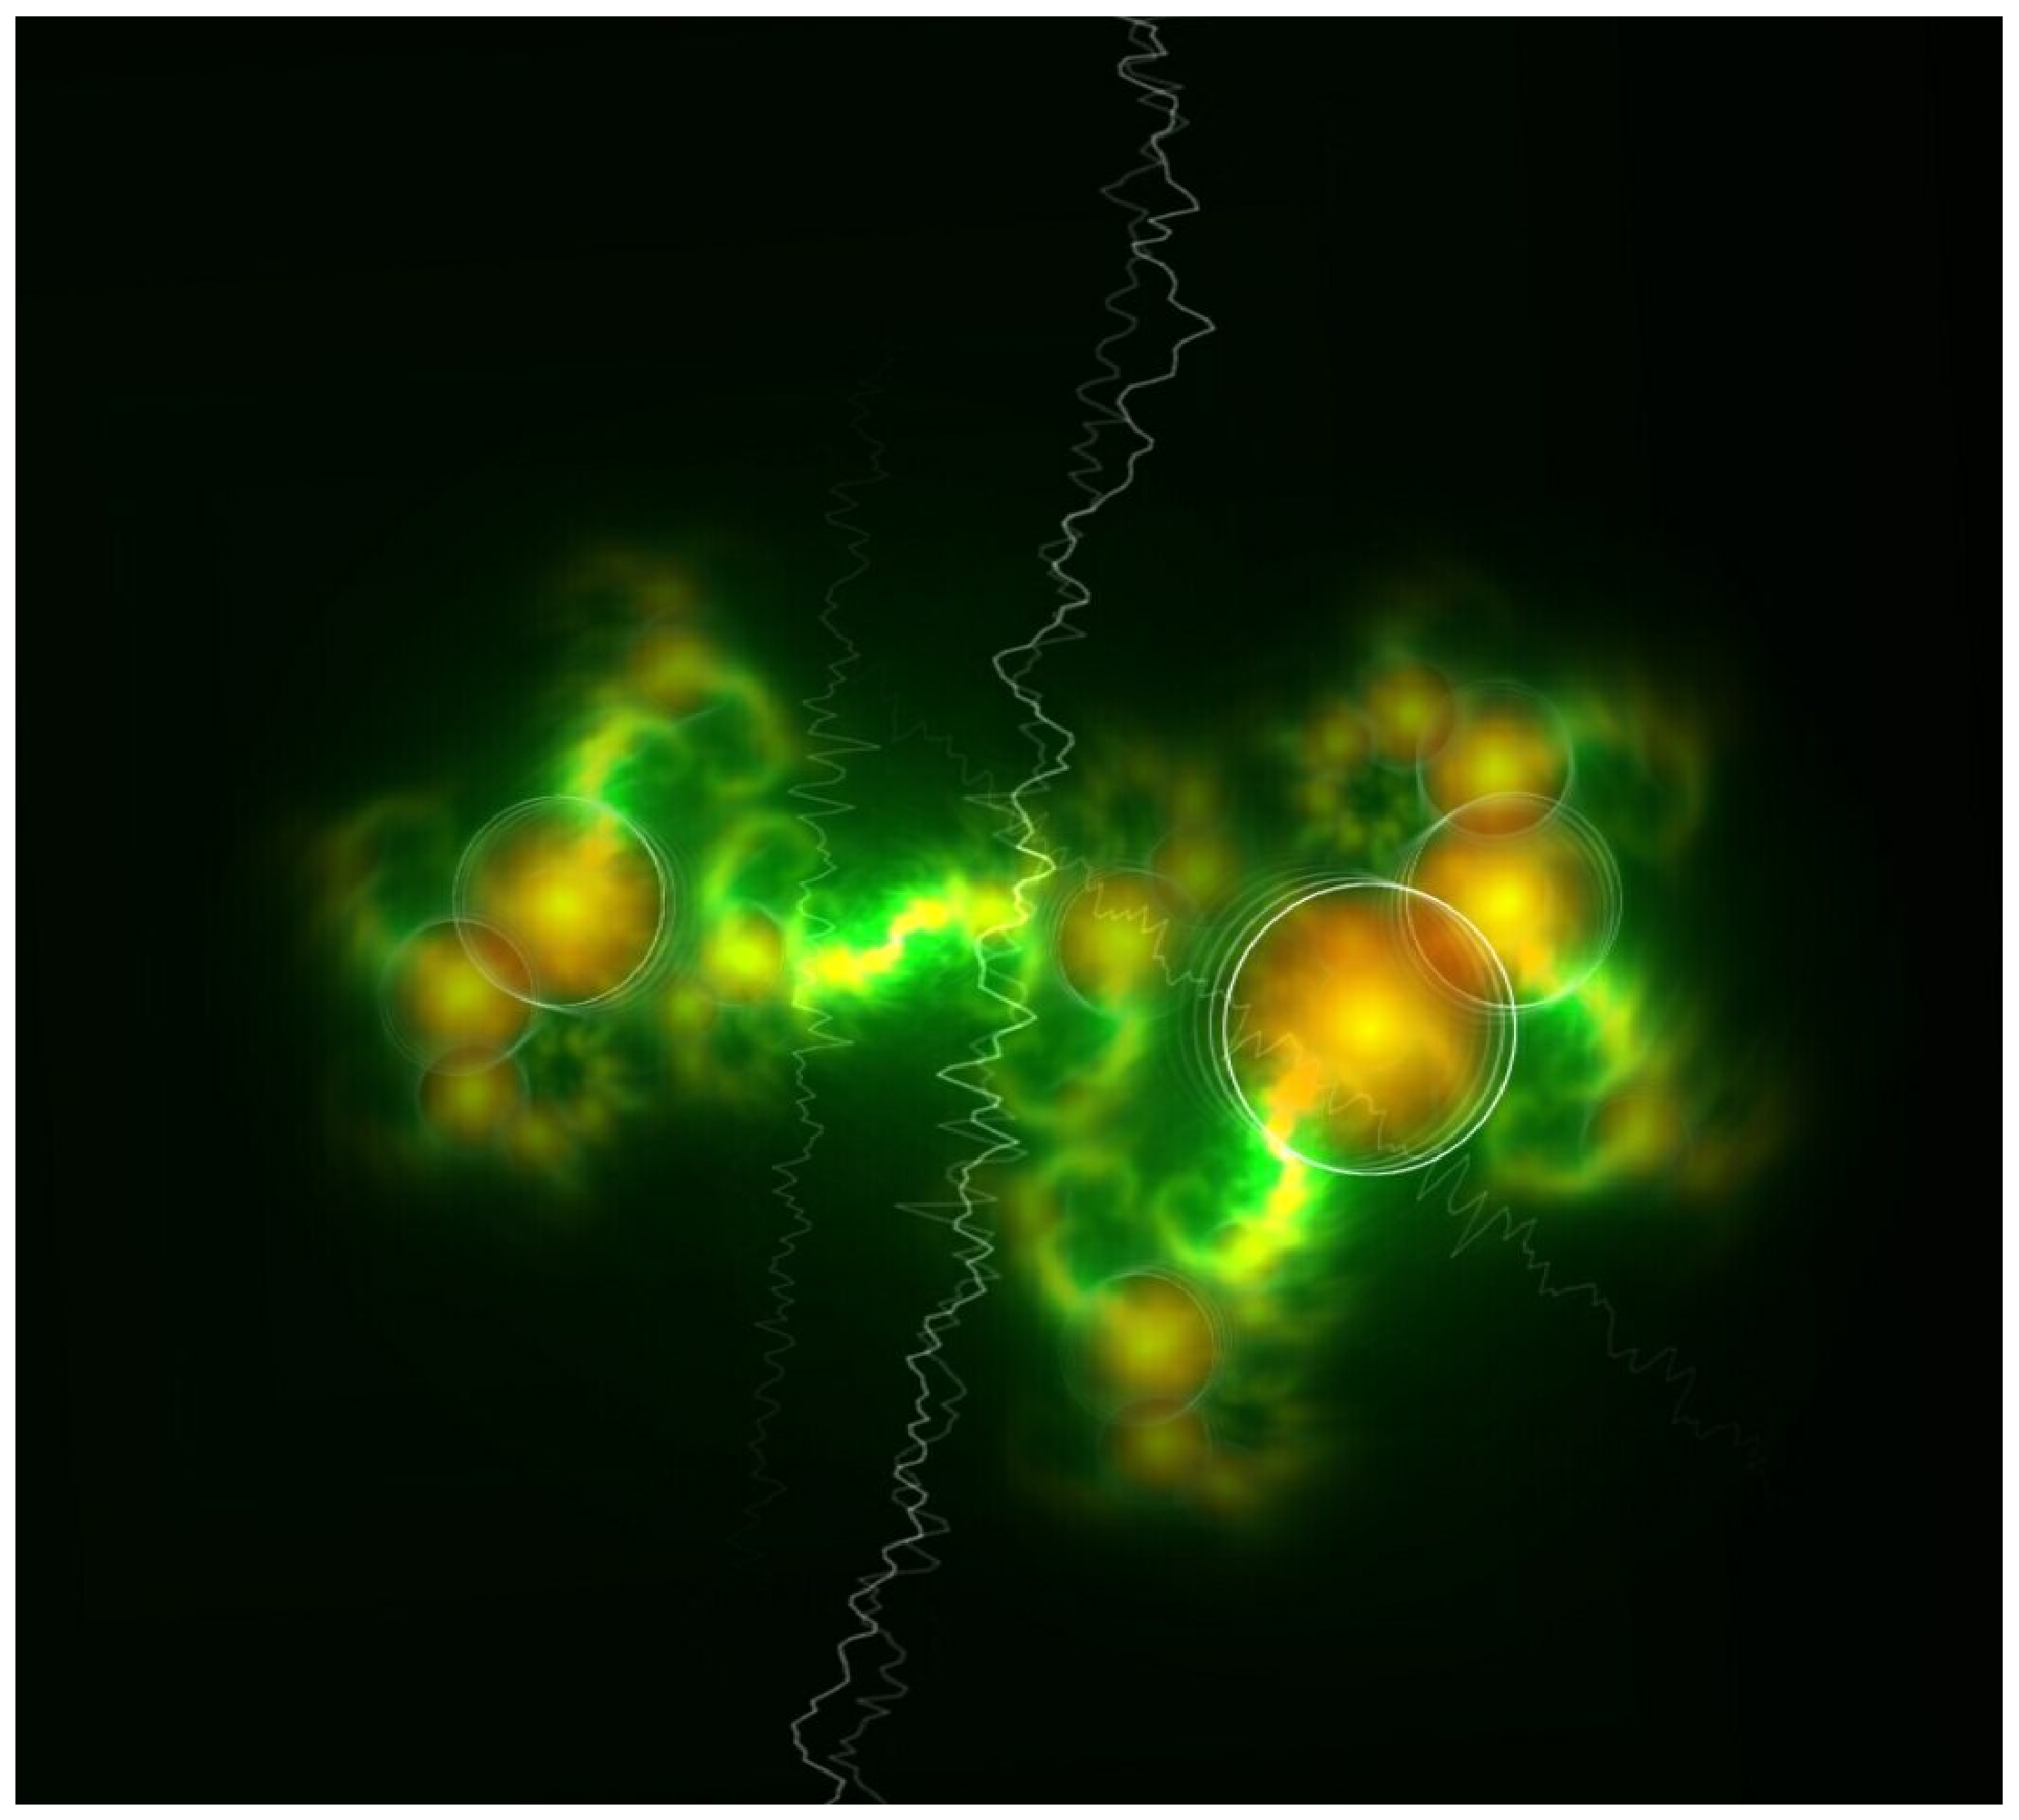
\includegraphics[height=58mm]{milkdrop1.eps}
  \end{figure}
}

\frame
{
  \frametitle{What is that MilkDrop thing?}
  \begin{figure}[H]
  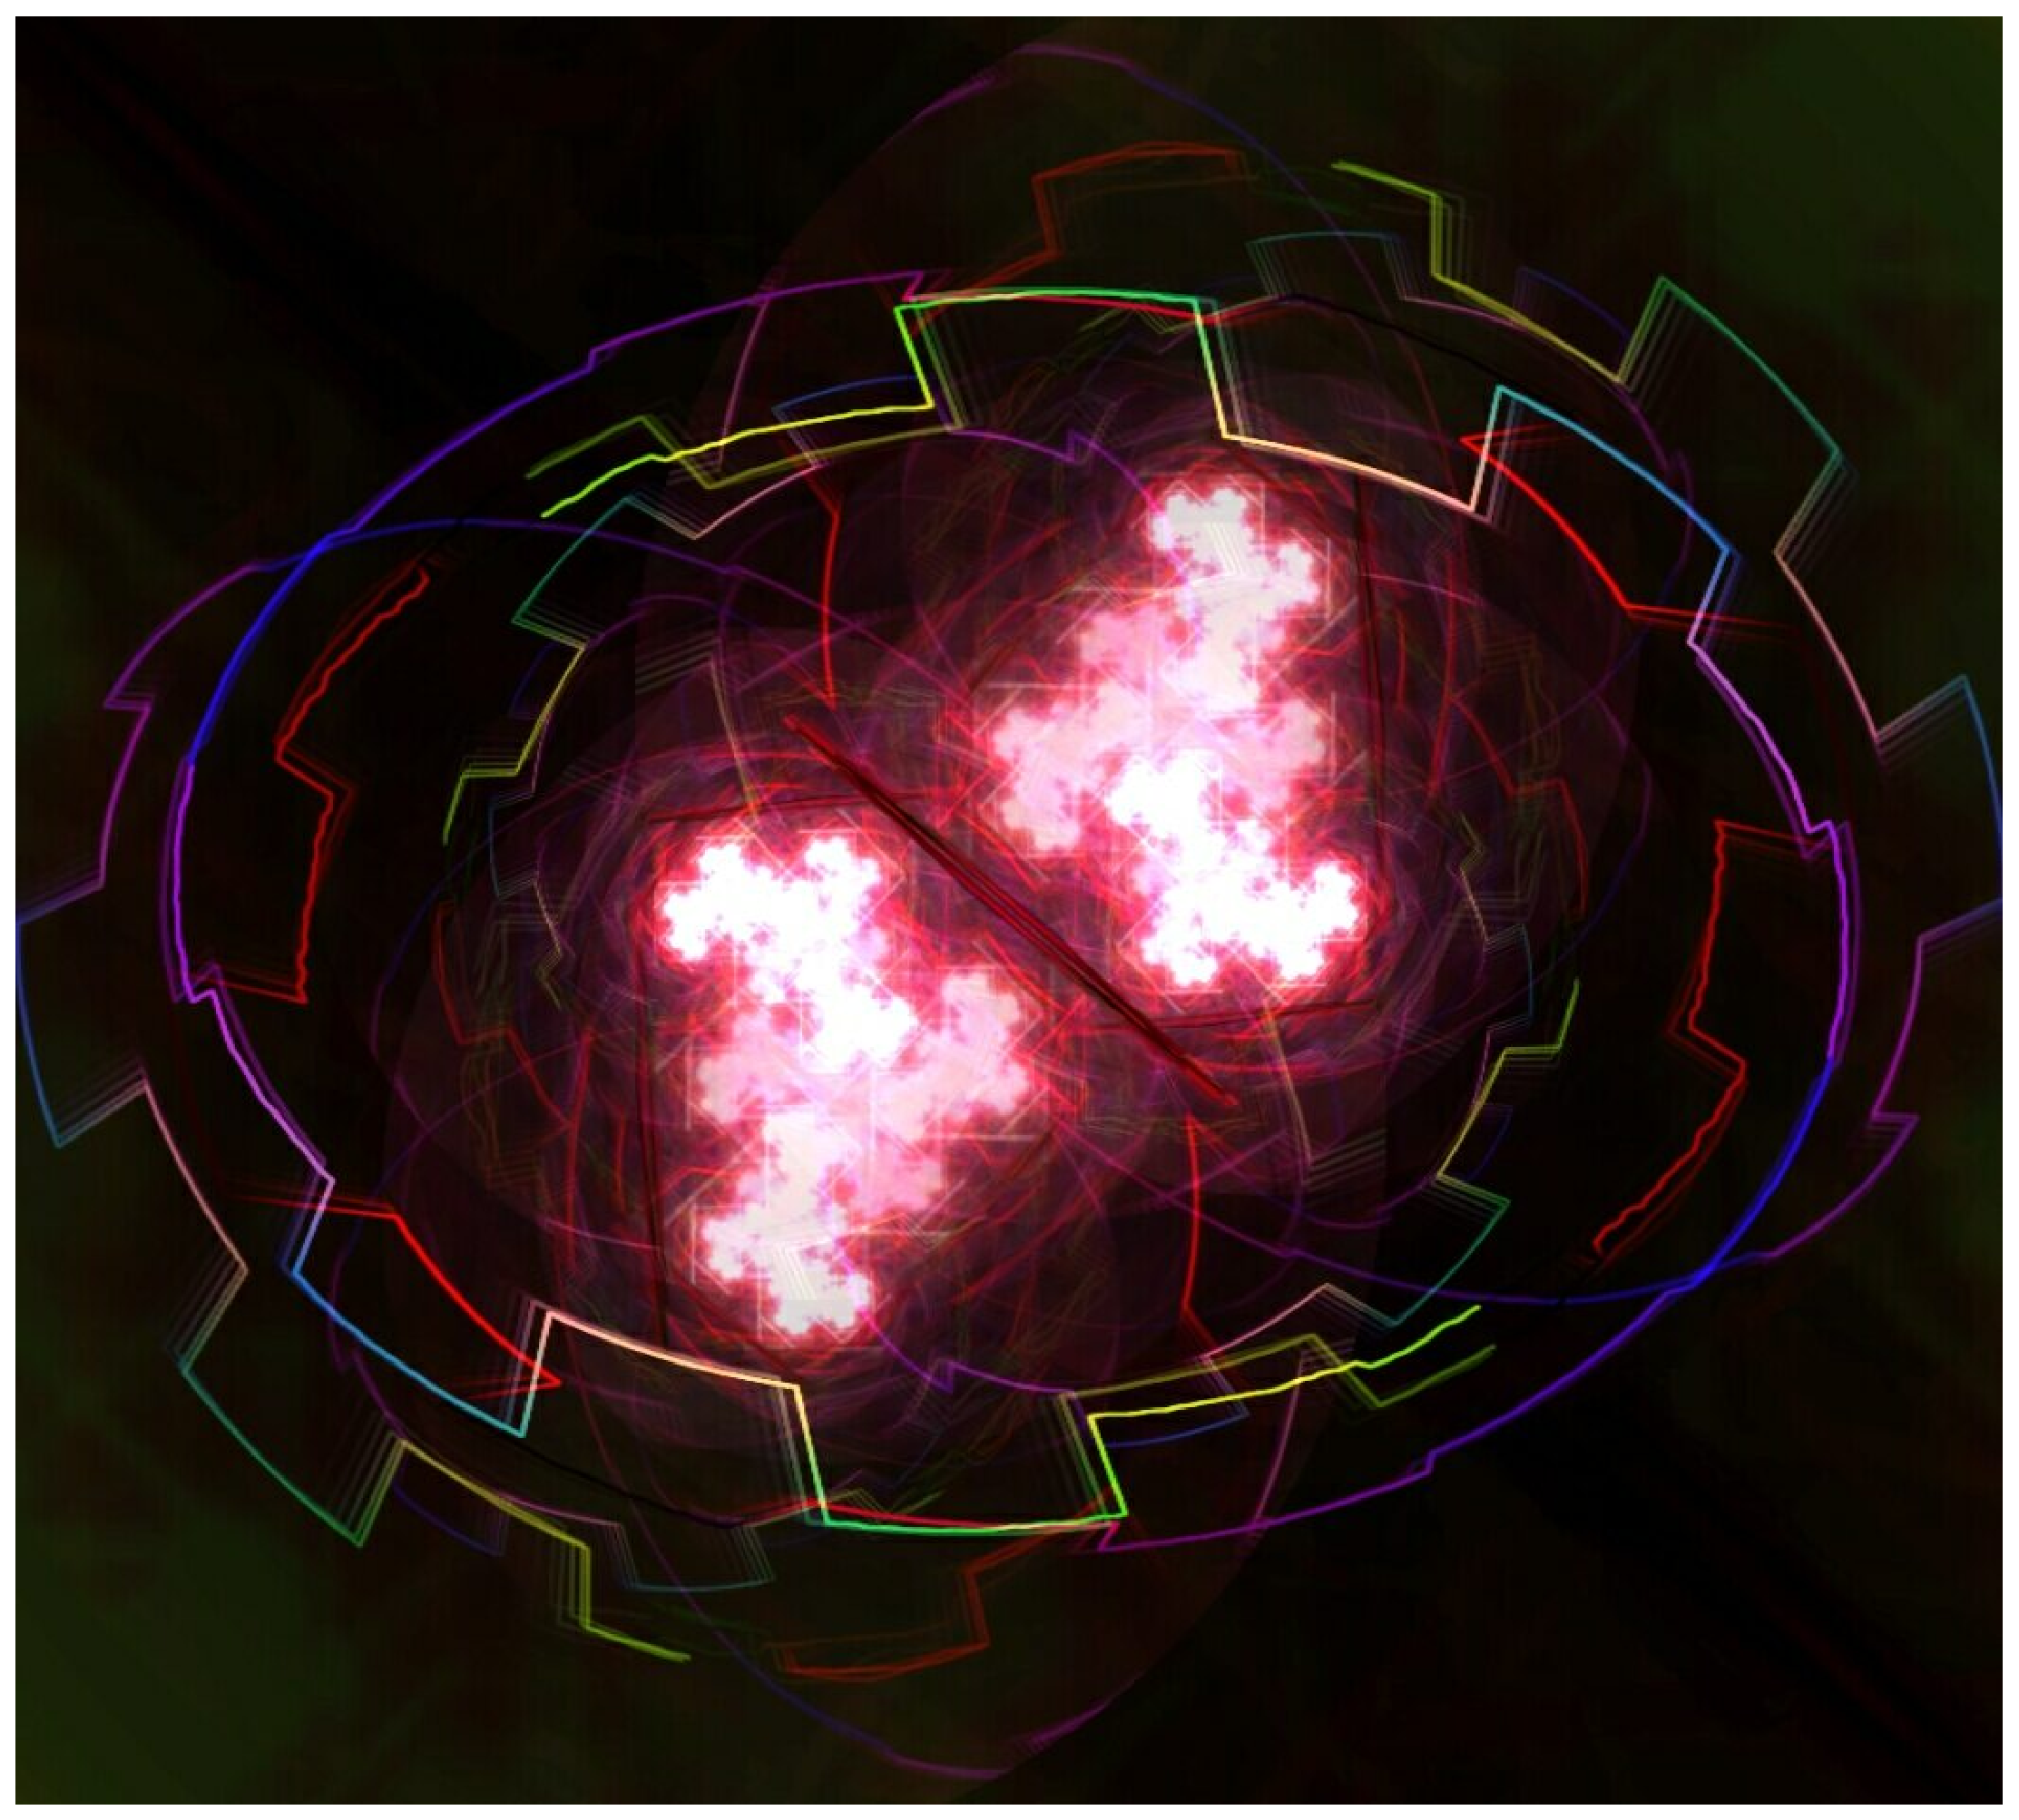
\includegraphics[height=58mm]{milkdrop2.eps}
  \end{figure}
}

\frame
{
  \frametitle{What is that MilkDrop thing?}
  \begin{figure}[H]
  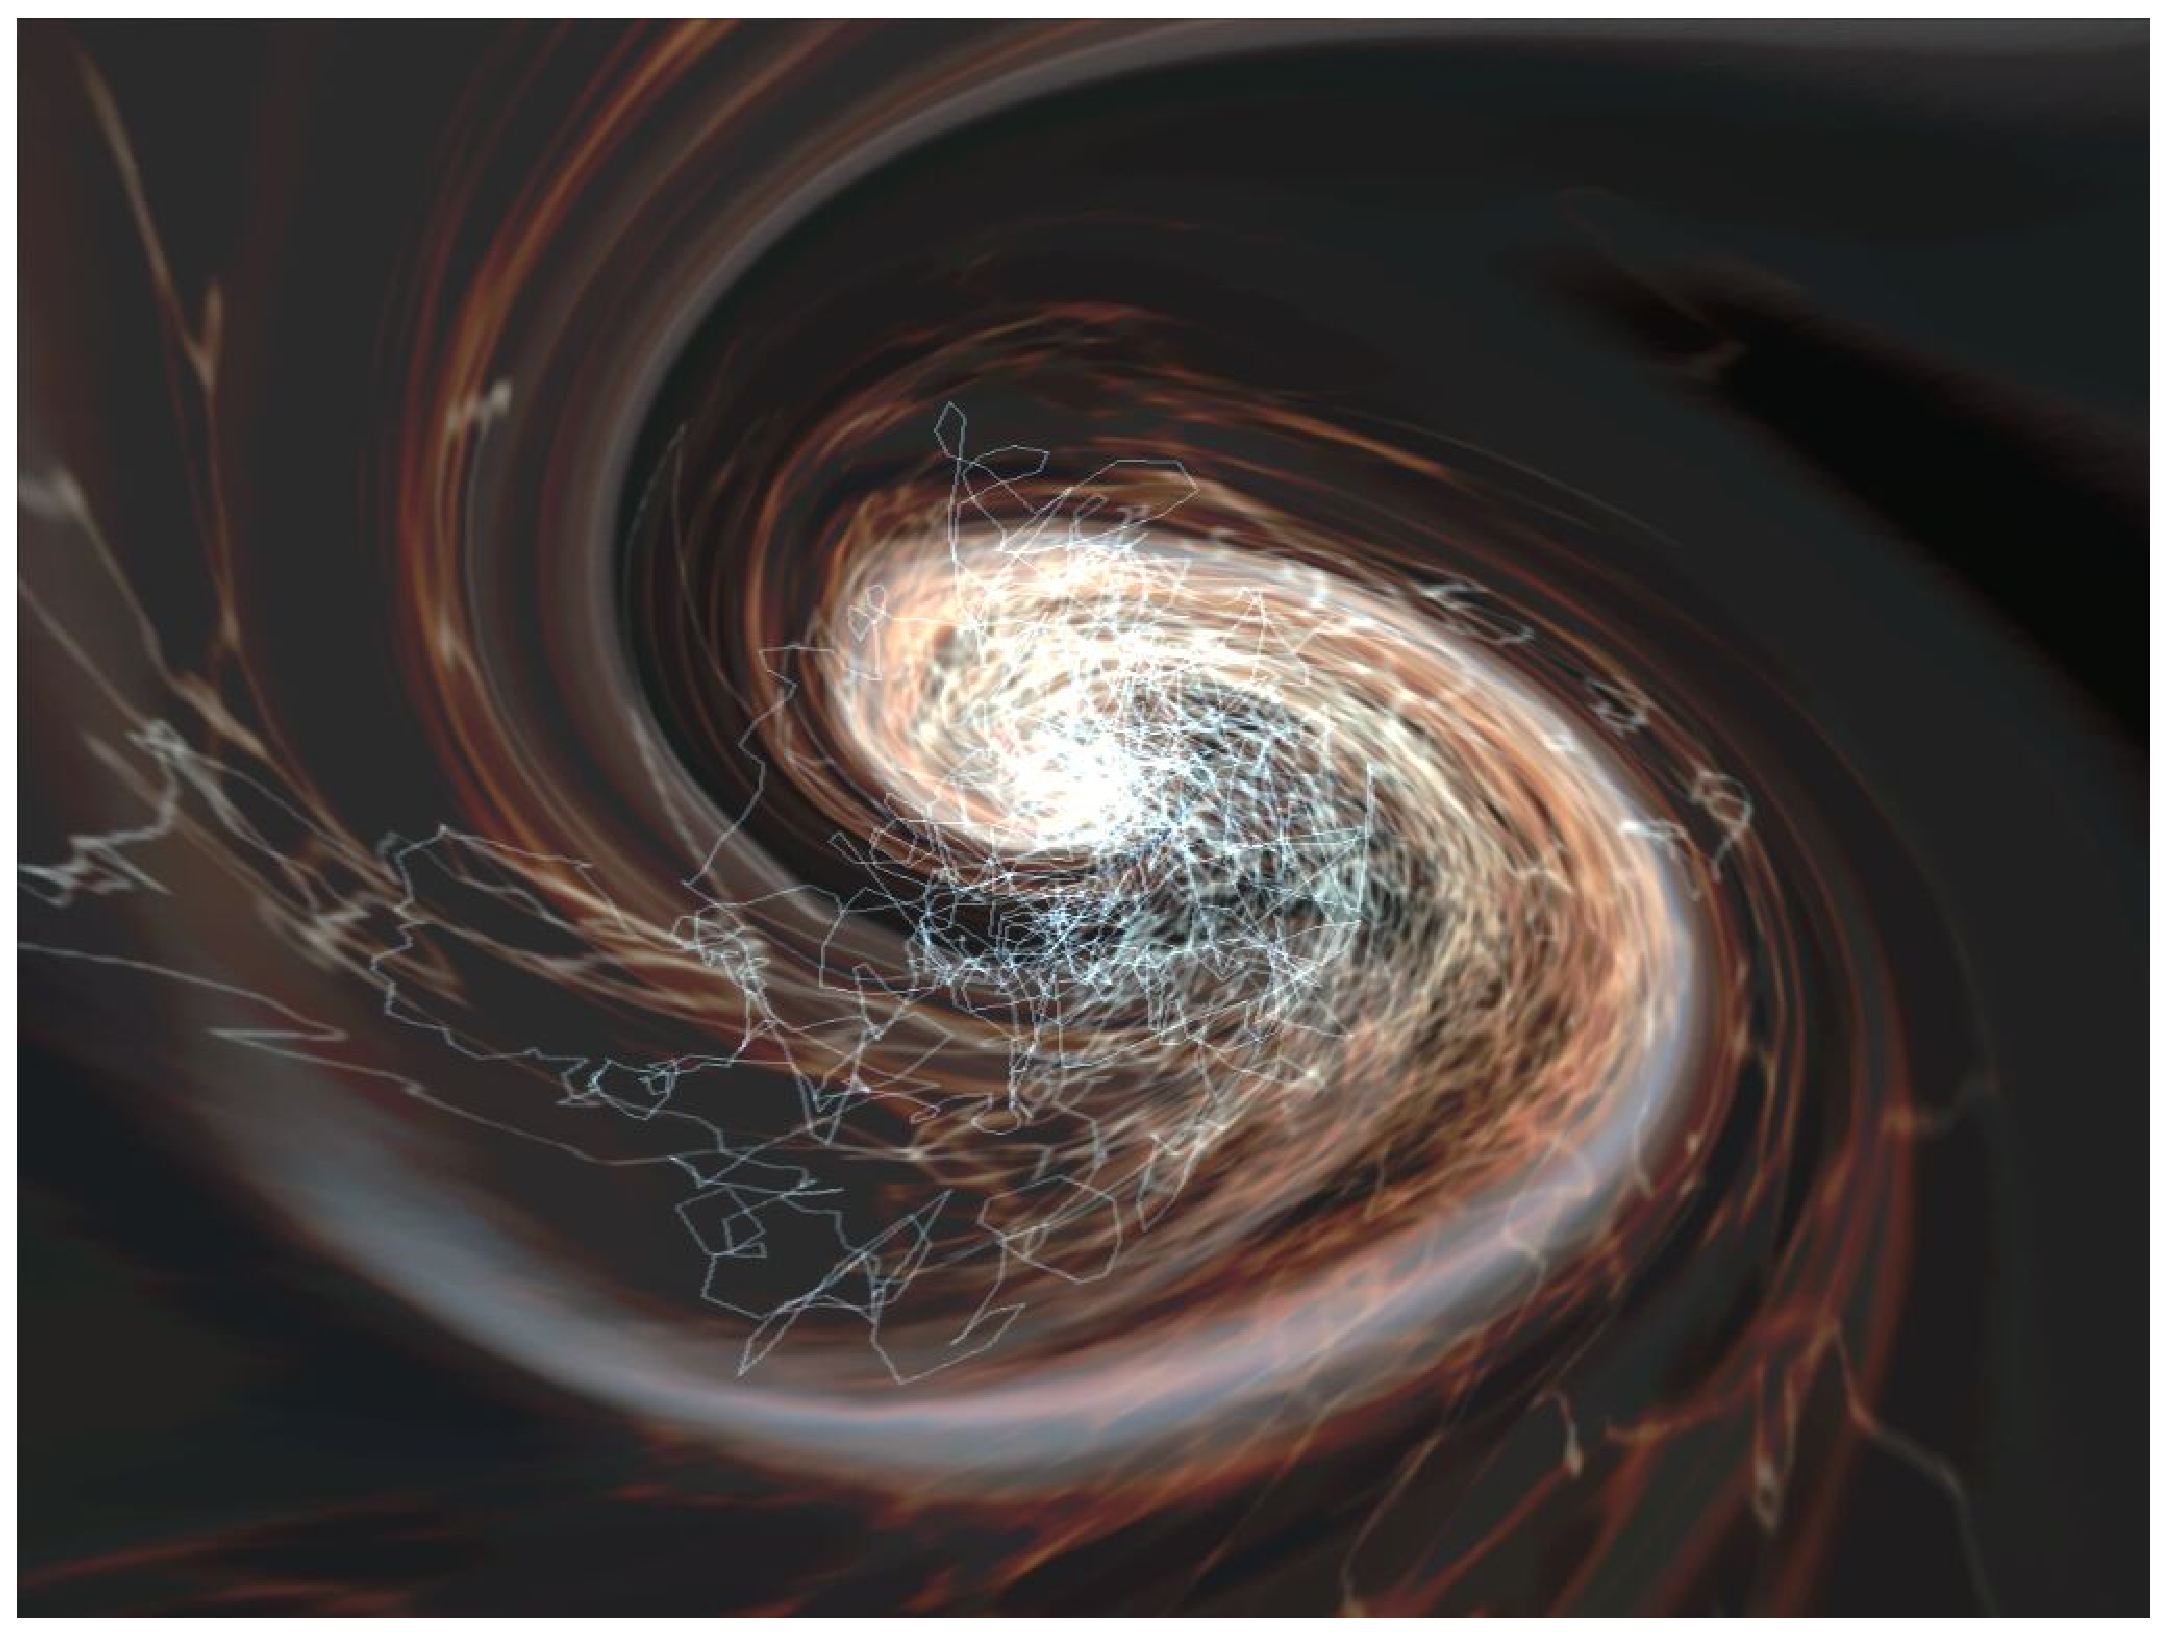
\includegraphics[height=58mm]{milkdrop3.eps}
  \end{figure}
}

\subsection{Open Hardware, for real}
\frame
{
  \frametitle{Open Hardware, for real}

  \begin{itemize}
  \item Arduino = AVR + power supply + connectors.
  \item The AVR chip does all the magic! And it's a black box in every sense.
  \item Here, all the logic of the chip is described (in Verilog HDL)...
  \item ...and open source!
  \item Ask Atmel for the same!
  \end{itemize}
}


\section{System architecture}
\subsection{The design flow}
\frame
{
  \frametitle{The design flow}
  
  ``System-on-a-Programmable-Chip'' (SoPC):
  \begin{itemize}
  \item A microcontroller is implemented using the FPGA fabric
  \item The software is written and compiled (GCC)
  \item The compiled firmware is flashed/loaded on the board
  \item The microprocessor made from the FPGA fabric executes it
  \item Acceleration units and specialty peripherals are added to the system and driven by the software
  \end{itemize}
}

\subsection{SoC interconnect}
\frame
{
  \frametitle{SoC interconnect}
  
  Three different buses are used:
  \begin{itemize}
  \item WISHBONE as general purpose bus (Opencores standard)
  \item Simplified bus for CSRs (custom)
  \item Fast Memory Link bus tailored for high speed DRAM access (custom)
  \end{itemize}
}

\subsection{Building blocks}
\frame
{
  \frametitle{Base system}
  
  \begin{itemize}
  \item 32-bit RISC CPU, WISHBONE bus, supported by GCC:
  \begin{itemize}
  \item Mico32 (from Lattice Semiconductors)
  \item AEMB (from Shawn Tan, instruction set compatible with Xilinx's Microblaze)
  \end{itemize}
  \item Off-chip Flash
  \item On-chip SRAM
  \item UART (debug), GPIO, ...
  \item Can run ucLinux or be programmed like a microcontroller, without OS.
  \end{itemize}
}

\frame
{
  \frametitle{Memory interface}
  
  \begin{itemize}
  \item Off-chip DDR SDRAM
  \item Custom controller
  \item Flexible and high quality
  \begin{itemize}
  \item reused by the NASA in the development of a software-defined radio prototype for the ISS
  \end{itemize}
  \item Custom high-performance bus interface (FML)
  \item Bridged to WISHBONE
  \begin{itemize}
  \item the base system can transparently access DRAM
  \end{itemize}
  \end{itemize}
}

\frame
{
  \frametitle{VGA output}
  
  \begin{itemize}
  \item The FPGA directly drives a video DAC for VGA
  \item Framebuffer-based (in DDR SDRAM)
  \item Supports multiple buffering
  \item Automatic buffer switch during blanking intervals
  \end{itemize}
}

\frame
{
  \frametitle{Graphics acceleration}
  
  \begin{itemize}
  \item Texture mapping unit
  \begin{itemize}
  \item implements any kind of image ``distortion''
  \end{itemize}
  \item Programmable floating point unit
  \begin{itemize}
  \item similar to a vertex shader
  \end{itemize}
  \item Flexible, can be used to implement MilkDrop or others...
  \end{itemize}
}

\frame
{
  \frametitle{Video inputs}
  
  \begin{itemize}
  \item Still in development
  \item Dual PAL/NTSC inputs
  \item Off-chip ADC and decoder
  \item For live video mixing applications
  \end{itemize}
}

\frame
{
  \frametitle{Control peripherals}
  
  \begin{itemize}
  \item Also in development
  \item Support planned for:
  \begin{itemize}
  \item MIDI (electronic instruments)
  \item DMX512 (stage lighting)
  \item Ethernet -- OpenSoundControl
  \end{itemize}
  \item Artistic installations, performances, ...
  \end{itemize}
}


\section{Contacts}
\frame
{
  \frametitle{Thank you for your attention}
  \begin{itemize}
  \item Web: \url{http://www.milkymist.org}
  \begin{itemize}
  \item documented source code (GPLv3 licensing)
  \item binary kits (to get started fast)
  \item mailing list
  \item wiki (with suggested contributions)
  \item blog
  \item these slides are online (GNU FDL licensing)
  \end{itemize}
  \item Mail: sebastien.bourdeauducq [AT] lekernel DOT net
  \end{itemize}

  \begin{center}
  \framebox[100mm][c]{Questions?}
  \end{center}
}

\end{document}
